\documentclass[a4paper,14pt]{extarticle}

% ===== ЯЗЫК И ШРИФТ =====
\usepackage{fontspec}
\usepackage{polyglossia}

% Основной текстовый шрифт
\setmainfont[
  Path=fonts/,
  UprightFont=times.ttf,
  BoldFont=timesbd.ttf,
  ItalicFont=timesi.ttf,
  BoldItalicFont=timesbi.ttf
]{Times New Roman}

% Явное назначение шрифта для кириллицы
\newfontfamily\cyrillicfont[
  Path=fonts/,
  Script=Cyrillic,
  UprightFont=times.ttf,
  BoldFont=timesbd.ttf,
  ItalicFont=timesi.ttf,
  BoldItalicFont=timesbi.ttf
]{Times New Roman}

% Моноширинный шрифт с поддержкой кириллицы
\setmonofont{DejaVu Sans Mono}

\newfontfamily\cyrillicfonttt[
  Script=Cyrillic
]{DejaVu Sans Mono}

% Основной язык документа
\setdefaultlanguage{russian}

% ===== СТРАНИЦЫ И АБЗАЦЫ =====
\usepackage[
  a4paper,
  left=30mm,
  right=10mm,
  top=20mm,
  bottom=20mm
]{geometry}

\usepackage{setspace}
\singlespacing

\setlength{\parindent}{0cm}
\setlength{\parskip}{0pt}
\raggedbottom

% ===== ФОРМУЛЫ И РИСУНКИ =====
\usepackage{amsmath}
\usepackage{amssymb}
\usepackage{graphicx}
\usepackage{pdfpages}
\usepackage{needspace}

% ===== КОММЕНТЫ =====
\usepackage{comment}

% ===== ЗАГОЛОВКИ =====
\newcommand{\heading}[1]{%
  \par
  \smallskip
  \Needspace{5\baselineskip}%
  \addvspace{\baselineskip}%
  {\centering\normalfont\normalsize #1\par}%
  \nobreak
  \vspace{0.5\baselineskip}%
  \nobreak
}

% ===== ПУНКТЫ РЕШЕНИЯ =====
\newcounter{solutionstep}

\newcommand{\step}[1]{%
  \par
  \Needspace{5\baselineskip}%
  \refstepcounter{solutionstep}%
  \addvspace{0.7\baselineskip}%
  \noindent\thesolutionstep\ #1
}

\begin{document}

% ===== ТИТУЛЬНЫЙ ЛИСТ =====
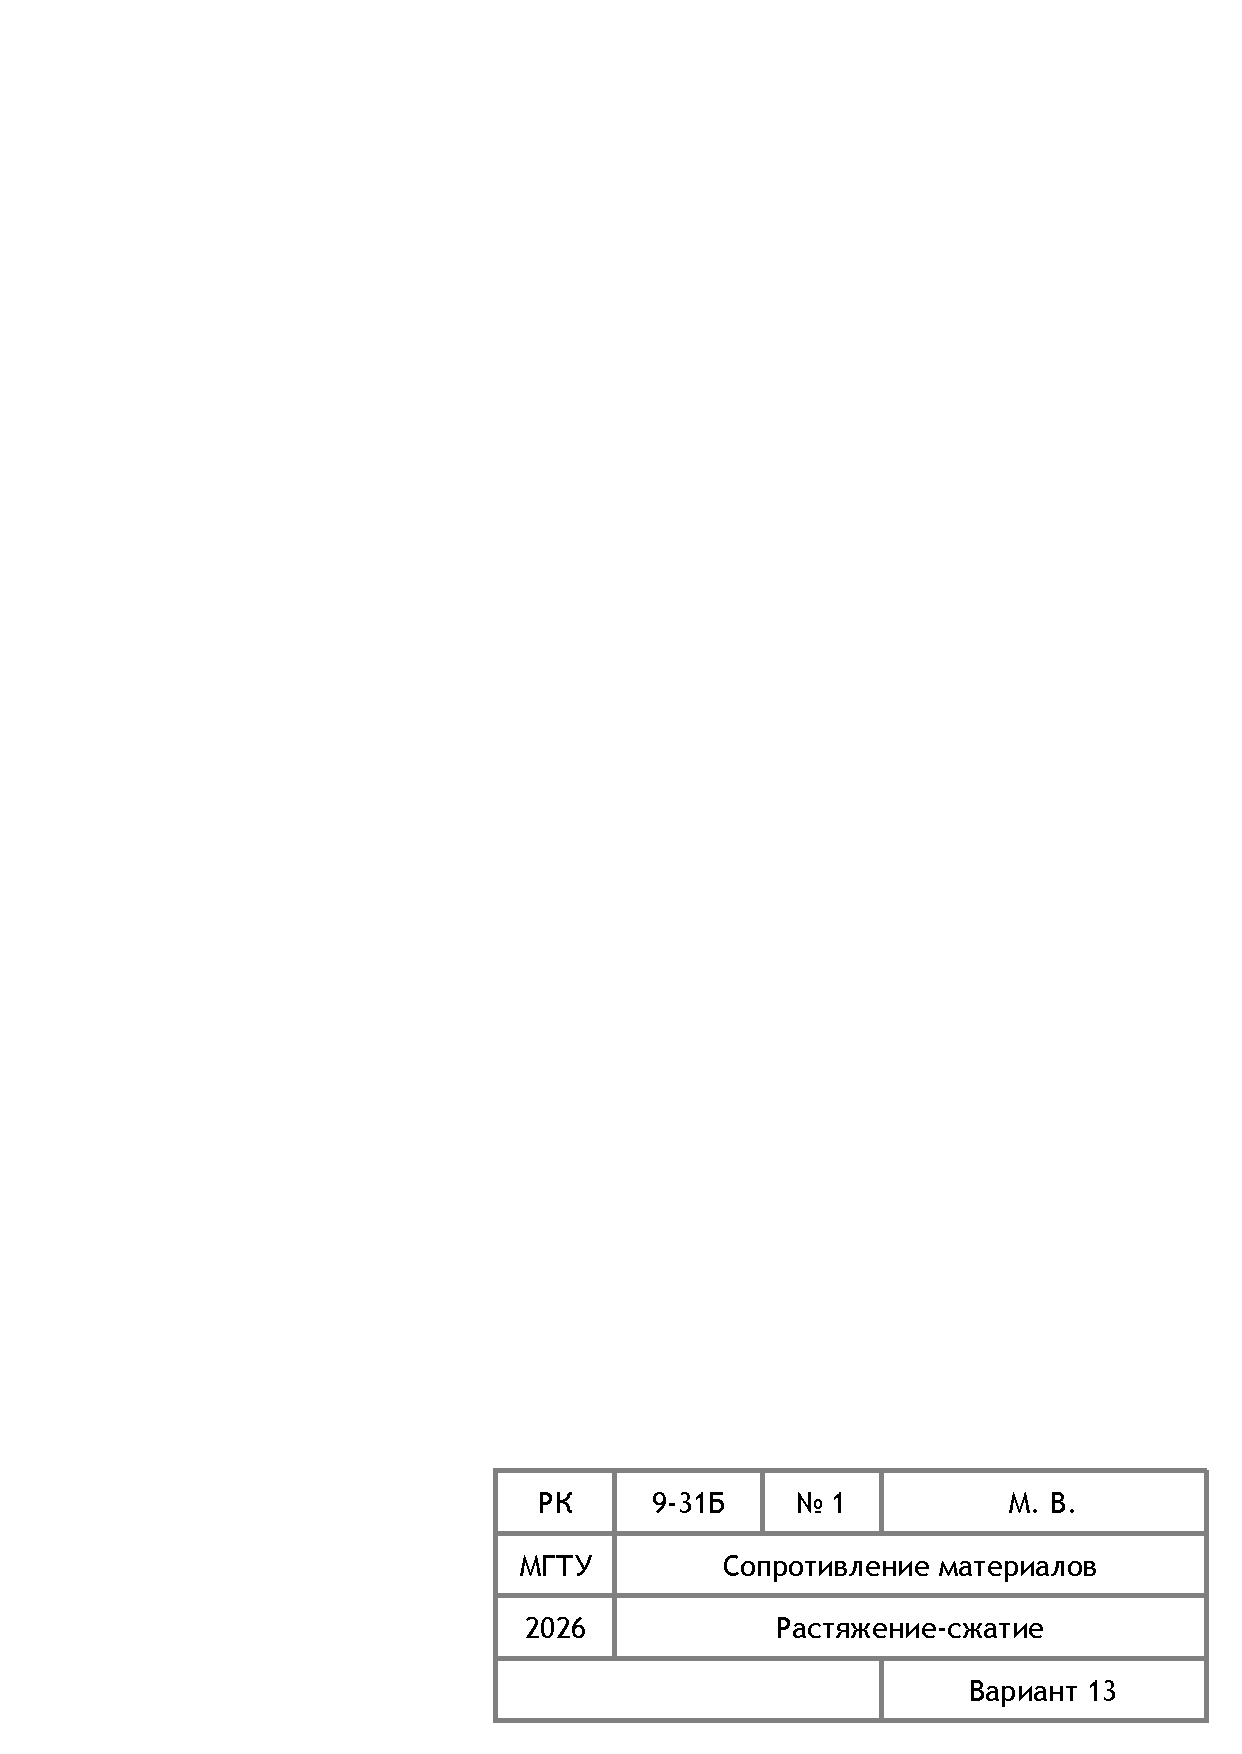
\includepdf[
  pages=1,
  noautoscale=true,
  pagecommand={\thispagestyle{empty}}
]{title.pdf}
% ===== ЗАДАЧА 1 =====
\heading{ЗАДАЧА 1}

\heading{УСЛОВИЕ}


Построить эпюры продольной силы \(N\),
 \(\sigma\), \(w\)
 
\begin{center}
  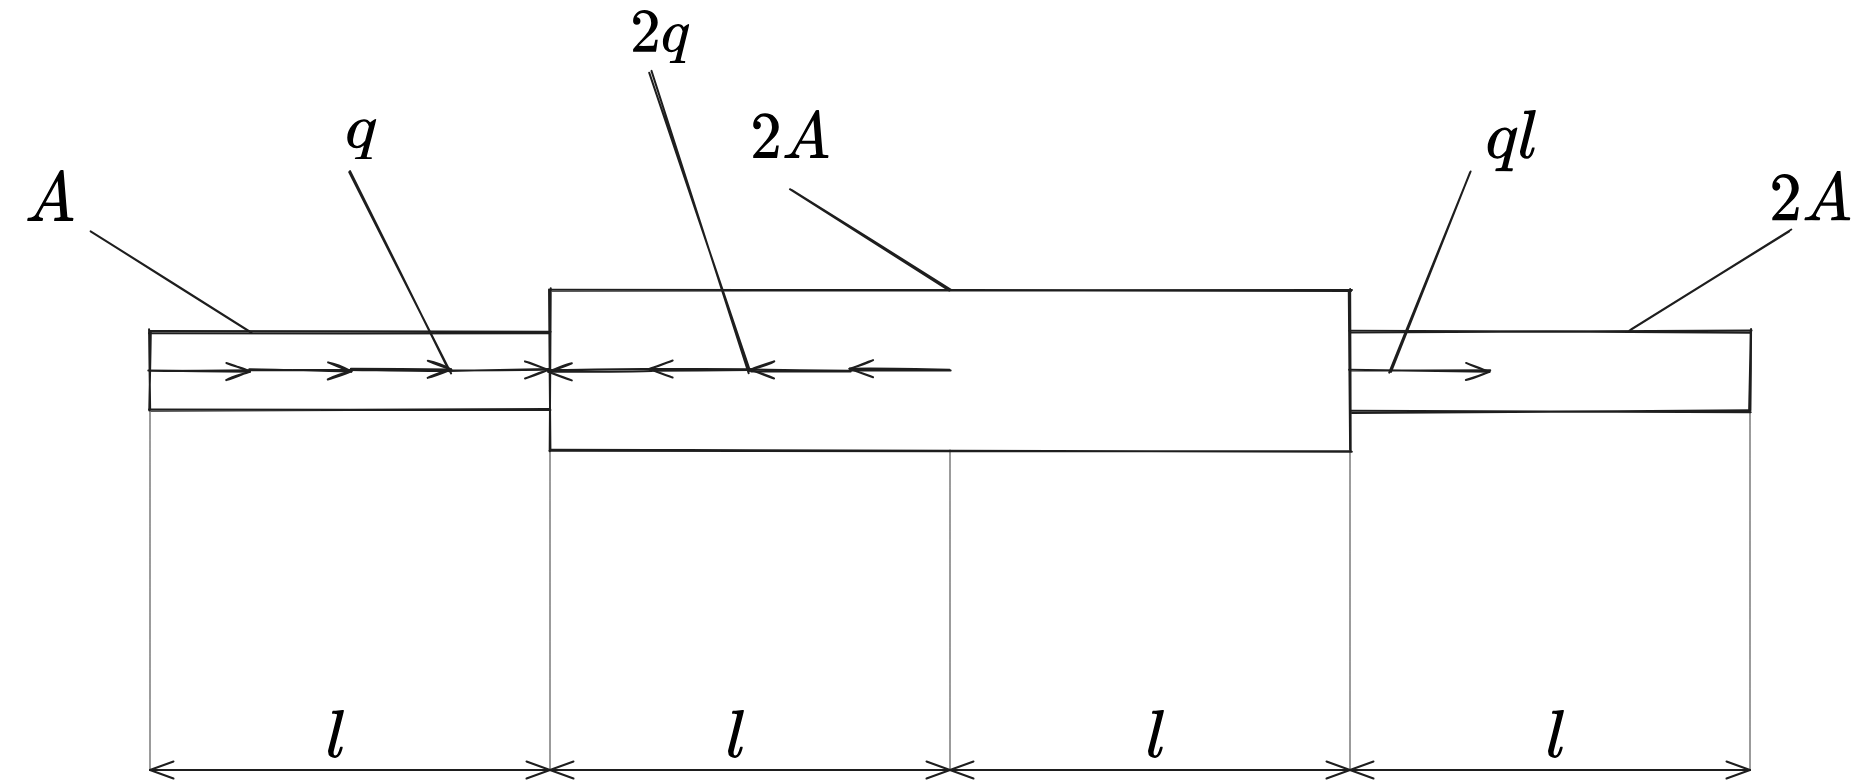
\includegraphics[
    width=0.90\linewidth,
    height=0.4\textheight,
    keepaspectratio
  ]{figures/task1_condition.png}
\end{center}
\heading{РЕШЕНИЕ}
\setcounter{solutionstep}{0}

\step{Запишем уравнение равновесия}

\begin{equation*}
  ql-2ql+ql = 0.
\end{equation*}

\clearpage

\step{Построим эпюры}

\begin{center}
  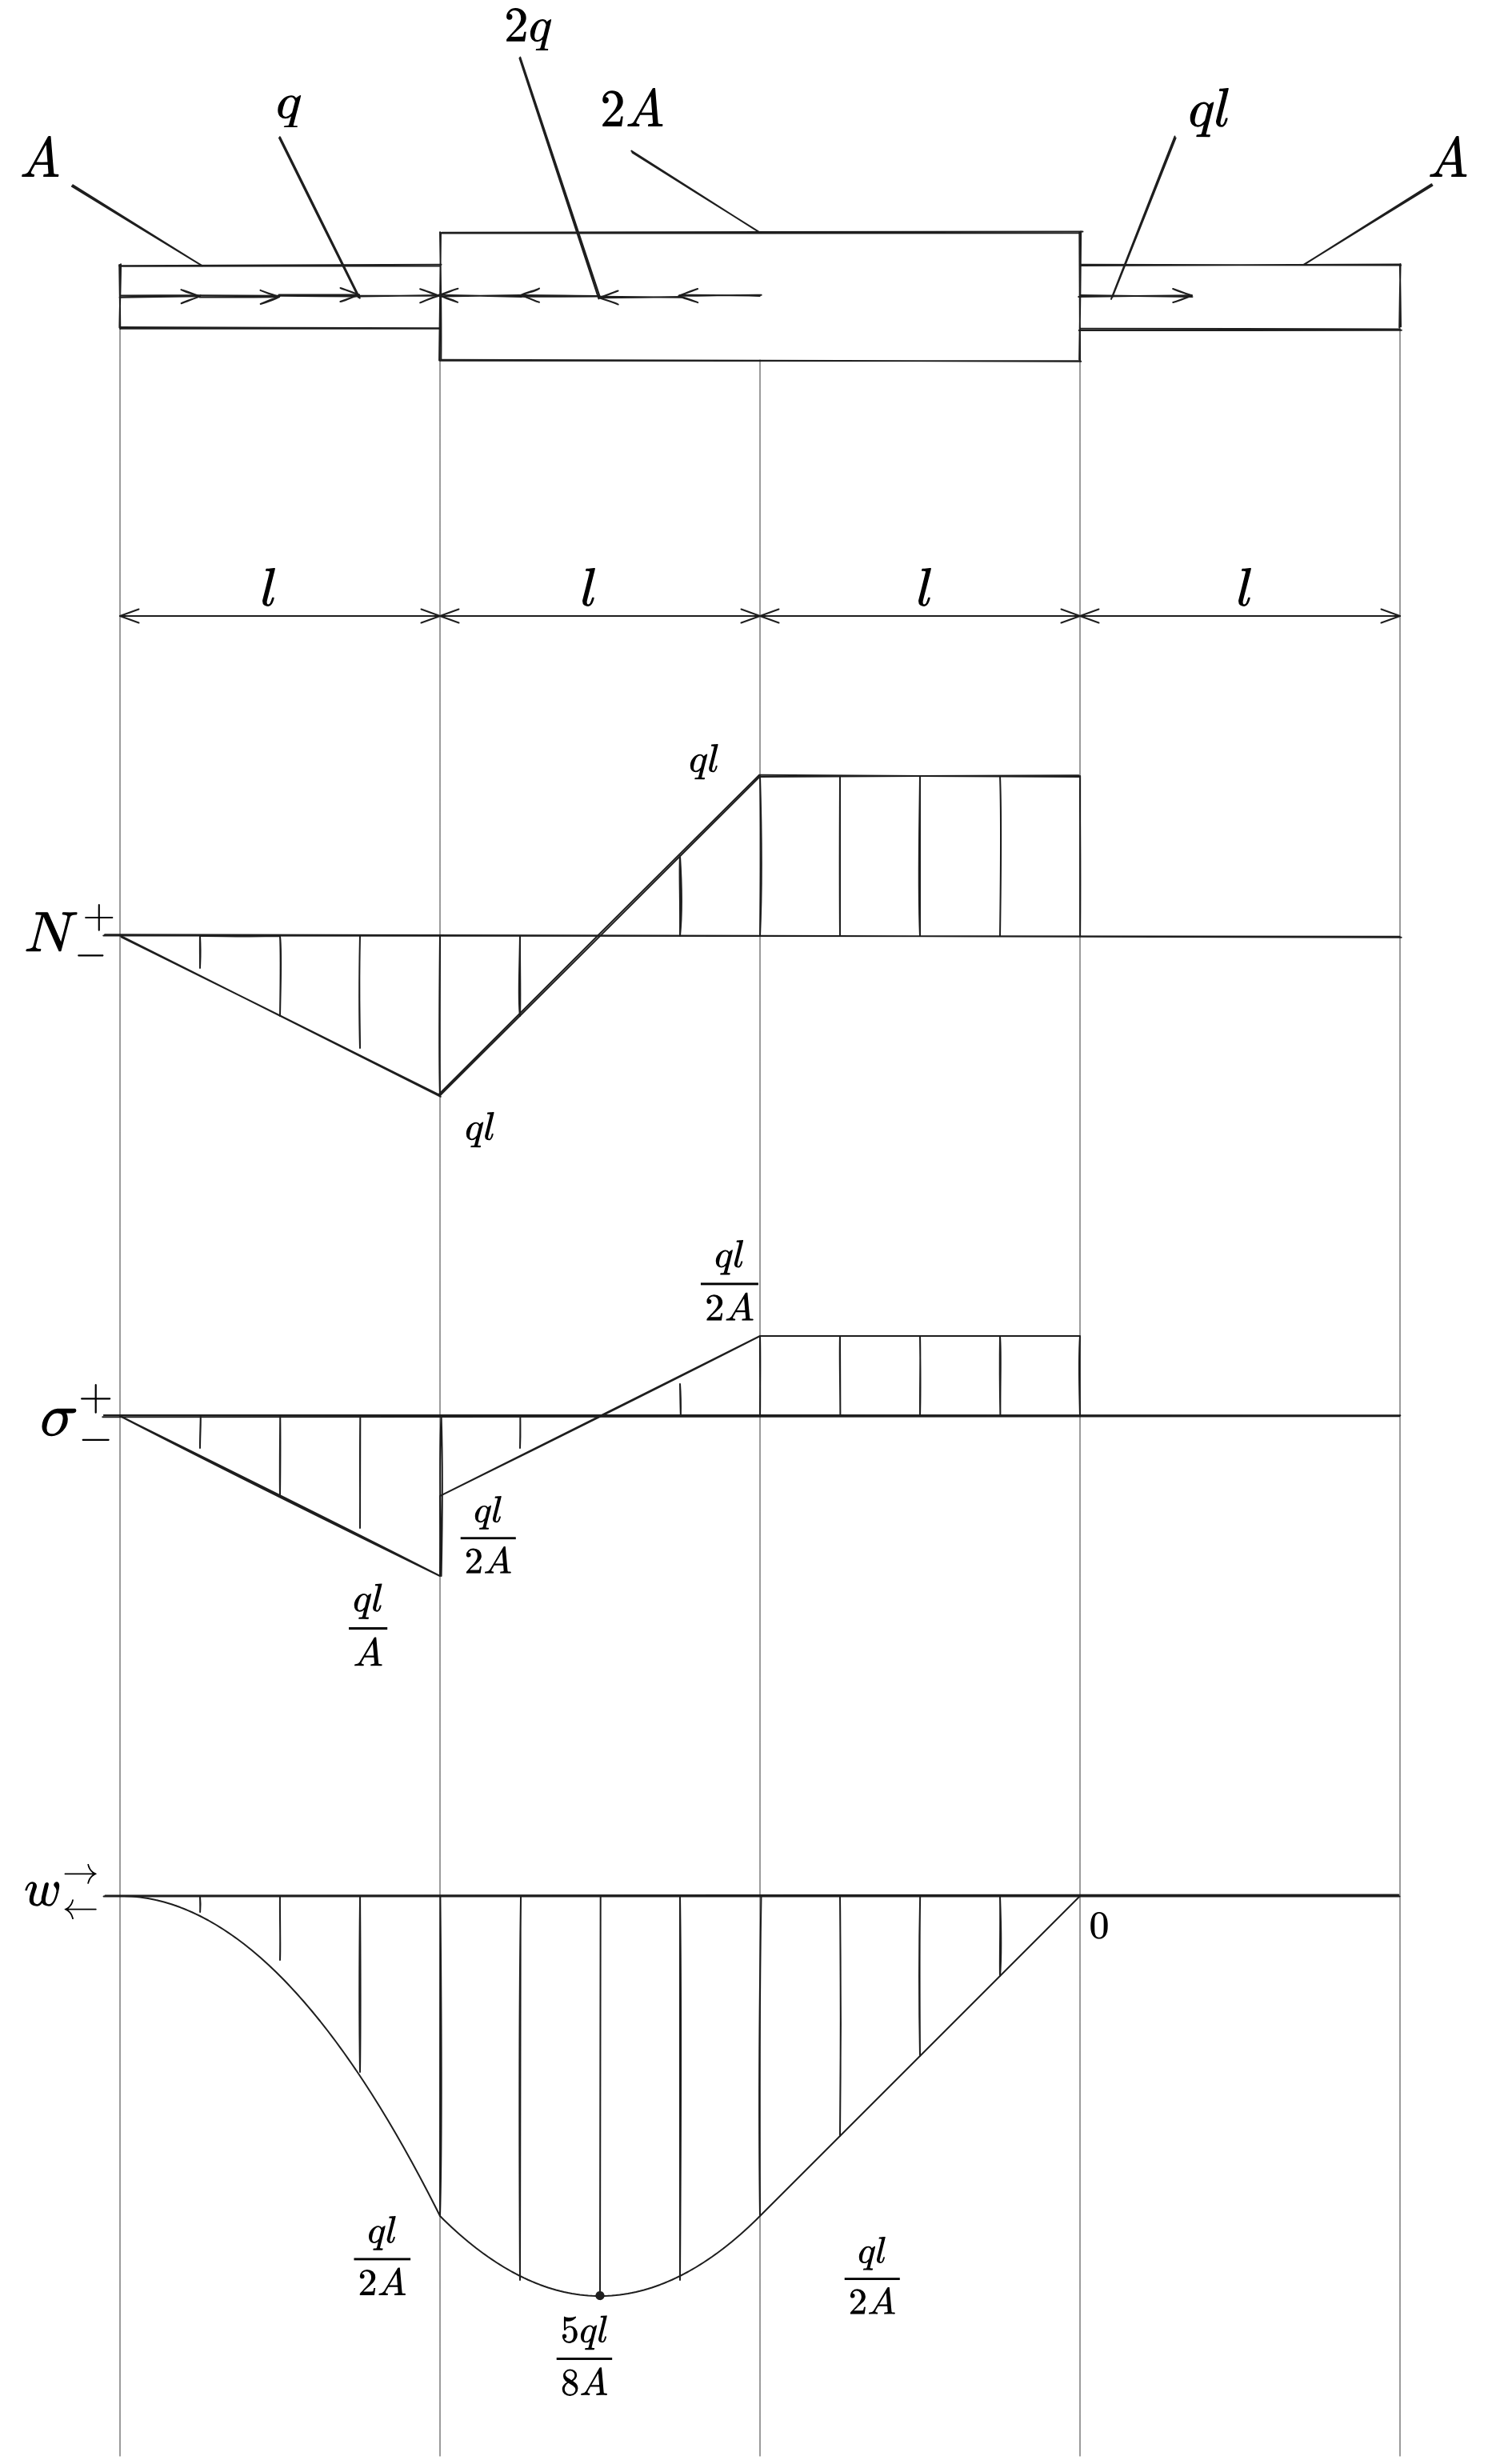
\includegraphics[
    width=0.90\linewidth,
    height=0.9\textheight,
    keepaspectratio
  ]{figures/task1_apure.png}
\end{center}

% ===== ЗАДАЧА 2 =====
\clearpage
\heading{ЗАДАЧА 2}

\heading{УСЛОВИЕ}

Между стержнями имеется зазор \(\delta=0{,}01\) мм. Участок \(BC\) нагревается на \(\Delta T\).
\begin{equation*}
l=150 \text{ мм},\quad E=2\cdot 10^5 \text{ МПа},\quad A=400\text{ мм}^2,
\end{equation*}
\begin{equation*}
\alpha=12\cdot10^{-6}\text{ 1/град},\quad \Delta T=100^\circ C
\end{equation*}

1 Построить эпюры \(N,\sigma,w\) при заданных параметрах

2 При каком \(\delta\) величина максимального напряжения равна 100 МПа?

\begin{center}
  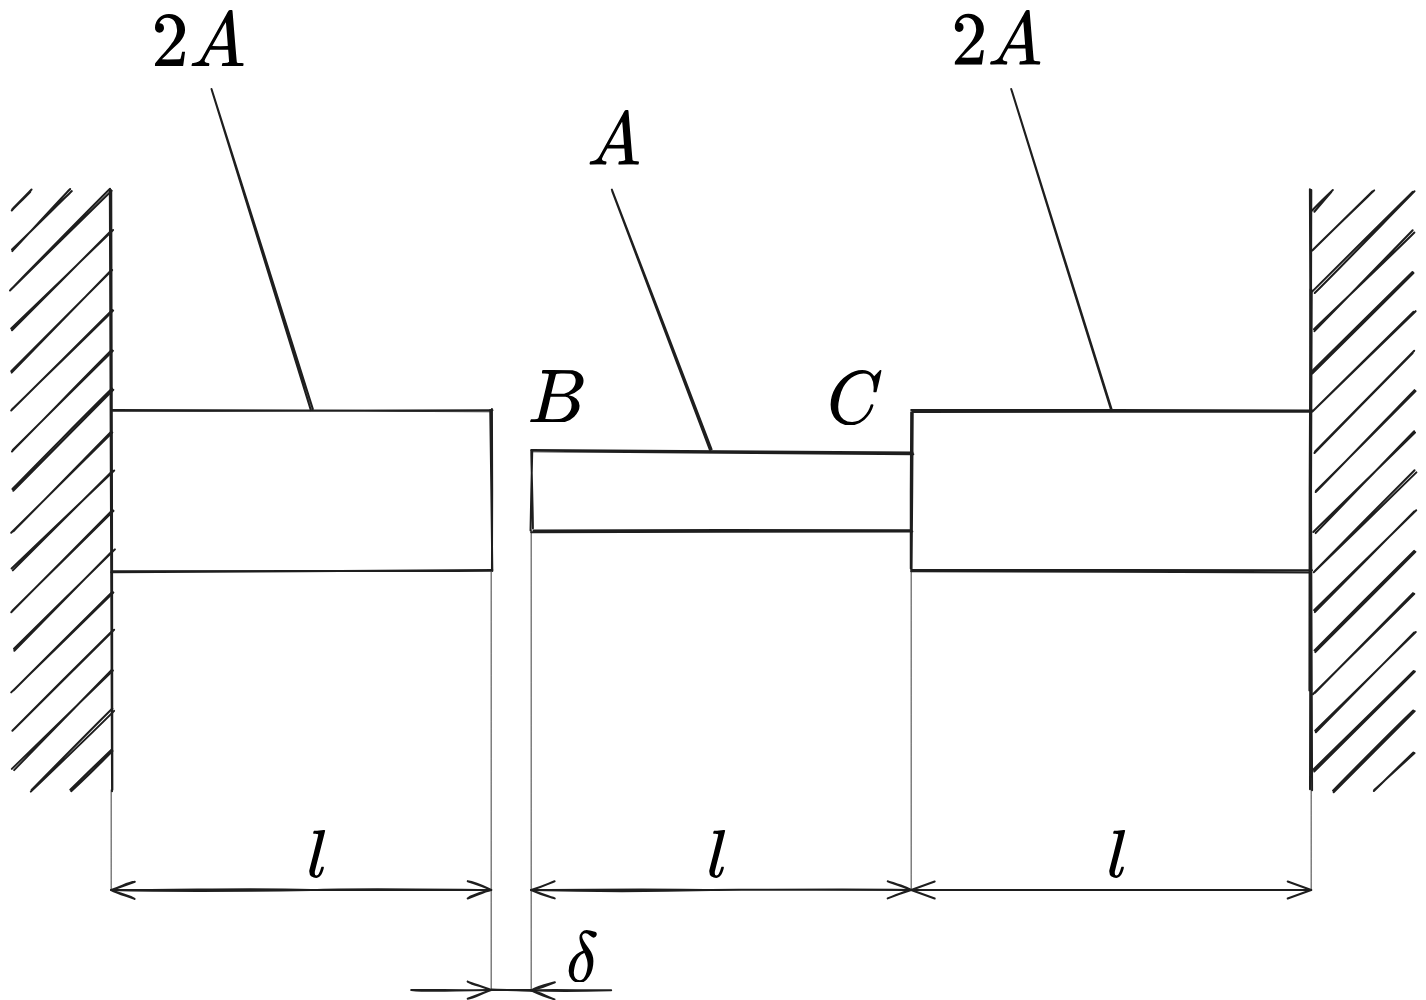
\includegraphics[
    width=0.90\linewidth,
    height=0.35\textheight,
    keepaspectratio
  ]{figures/task2_conditions.png}
\end{center}

\heading{РЕШЕНИЕ}
\setcounter{solutionstep}{0}
\step{Проверка закрытия зазора}
\begin{align*}
\Delta l_{BC}&=\alpha\Delta T l \\ 
\text{?: }\delta&\leq\alpha\Delta T l \\
0{,}01 \text{ мм} &\leq 12\cdot10^{-6}\text{ град}^{-1}\, \cdot100 ^\circ C \cdot 150 \text{ мм}\\ 
0{,}01 \text{ мм} &\leq 0{,}18 \text{ мм}
\end{align*}
Зазор закрывается
\clearpage

\step{Определение внутренних силовых факторов}

После закрытия зазора система статически неопределима, поэтому введем локальные координаты и найдем ВСФ через уравнения перемещения
\begin{center}
  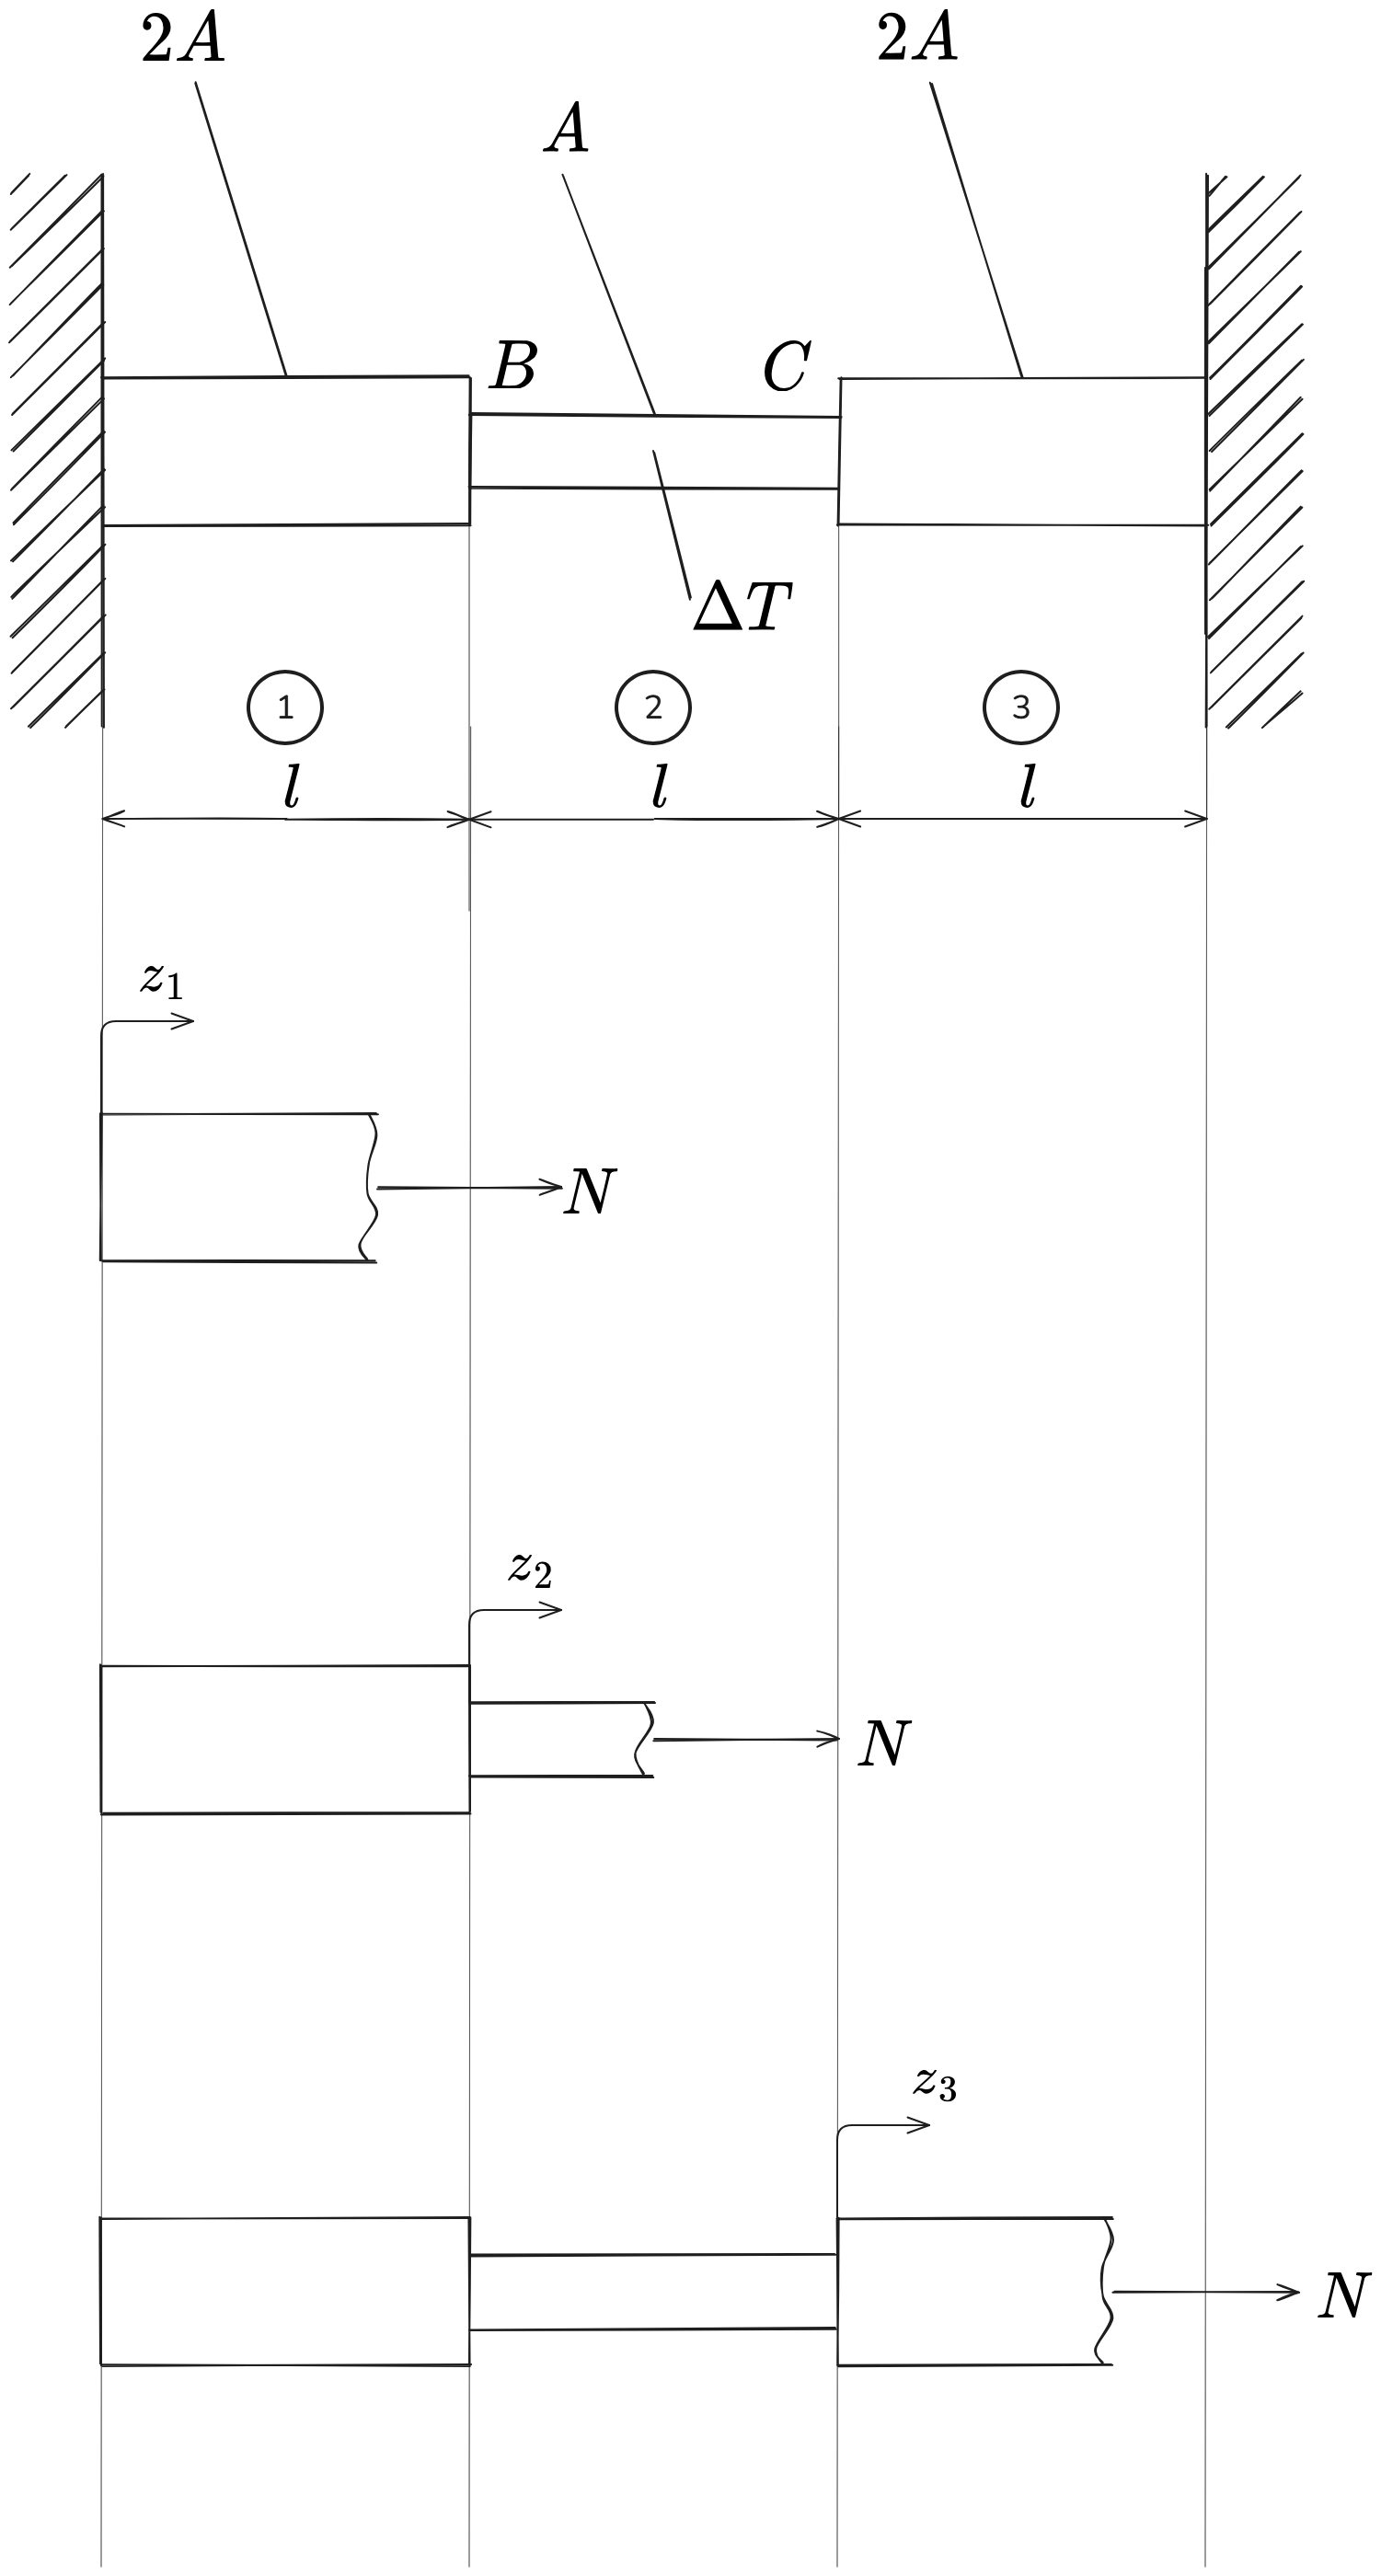
\includegraphics[
    width=1\linewidth,
    height=0.9\textheight,
    keepaspectratio
  ]{figures/task2_ISF.png}
\end{center}

\begin{equation*}
  \frac{Nl}{2AE}+\frac{Nl}{AE}+\alpha\Delta T l+\frac{Nl}{2AE}=\delta
\end{equation*}
\begin{equation*}
  N=(\delta-\alpha\Delta T l)\frac{AE}{2l}
\end{equation*}

Произведенм замену:
\(
k=\alpha\Delta T l -\delta\quad\implies\quad N=-k\frac{AE}{2l}
\)
\step{Определение напряжений}

\begin{equation*}
\sigma_1=\frac{N}{2A}=-k\frac{E}{4l}
\end{equation*}
\begin{equation*}
\sigma_2=\frac{N}{A}=-k\frac{E}{2l}
\end{equation*}
\begin{equation*}
\sigma_3=\frac{N}{2A}=-k\frac{E}{4l}
\end{equation*}

\step{Определение перемещений}
Для участка 1 координата \(z_1\) от левого края тела (\(0\leq z_1\leq l\))
\[
w_1(z_1)=\dfrac{N{z_1}}{2EA} \implies   w_1(l)=-\frac{1}{4}k
\]
Для участка 2 координата \(z_2\) от правого края участка 1 (\(0\leq z_2\leq l\))
\[
w_2(z_2)=w_1(l)-\delta+\dfrac{N{z_2}}{EA}+\alpha\Delta T z_2\implies w_2(l)=\frac{1}{4}k
\]
Для участка 3 координата \(z_3\) от правого края участка 2 (\(0\leq z_3\leq l\))
\[
w_3(z_3)=w_2(l)+\dfrac{N{z_3}}{2EA}\implies w_3(l)=0
\]

\step{Численный рассчет \(N,\sigma,w\)}
{\setlength{\jot}{8pt}
\begin{align*}
k&=\alpha\Delta T\,l-\delta=12\cdot10^{-6}\,\text{град}^{-1}
\cdot100\,\text{град}\cdot150\,\text{мм}-0{,}01\,\text{мм}\\
k&=0{,}17\,\text{мм}\\
N&=-k\frac{AE}{2l}
=-\frac{
2\cdot10^5\,\text{МПа}\cdot400\,\text{мм}^2
\cdot0{,}17\,\text{мм}
}{
2\cdot150\,\text{мм}
}\approx-45333{,}3\,\text{Н}\\
\sigma_1&=\sigma_3=\frac{N}{2A}
=\frac{-45333{,}3\,\text{Н}}{2\cdot 400\,\text{мм}^2}
\approx-56{,}7\,\text{МПа}\\
\sigma_2&=\frac{N}{A}
=\frac{
-45333{,}3\,\text{Н}
}{
400\,\text{мм}^2
}
\approx-113{,}3\,\text{МПа}\\
w_1(0)&=0\,\text{мм}\\
w_1(l)&=\frac{Nl}{2EA}=-\frac{k}{4}=-\frac{0{,}17\,\text{мм}}{4}=-0{,}0425\,\text{мм}\\
w_2(0)&=w_1(l)-\delta=-0{,}0425\,\text{мм}-0{,}01\,\text{мм}=-0{,}0525\,\text{мм}\\
w_2(l)&=w_2(0)+\frac{Nl}{EA}+\alpha\Delta T\,l=\frac{k}{4}=0{,}0425\,\text{мм}\\
w_3(0)&=w_2(l)=0{,}0425\,\text{мм}\\
w_3(l)&=w_3(0)+\frac{Nl}{2EA}=0\,\text{мм}
\end{align*}

}
\step{Определение зазора, при максимальном напряжении \(\sigma_{\max}=100\) МПа}
\begin{align*}
\sigma_{\max}&=-\sigma_2=k\frac{E}{2l}=(\alpha\Delta T l-\delta)\frac{E}{2l}\\
\delta&=\alpha\Delta T l-\frac{2l\,\sigma_{\max}}{E}\\
\delta
&=12\cdot10^{-6}\,\text{град}^{-1}
\cdot100\,\text{град}\cdot150\,\text{мм}
-\frac{100 \text{ МПа}\cdot 2\cdot 150\text{ мм}}{2\cdot10^5 \text{МПа}}
\\
\delta
&=0{,}18\,\text{мм}-0{,}15\,\text{мм}=0{,}03\,\text{мм}
\end{align*}

\clearpage

\step{Построение эпюр}

\begin{center}
  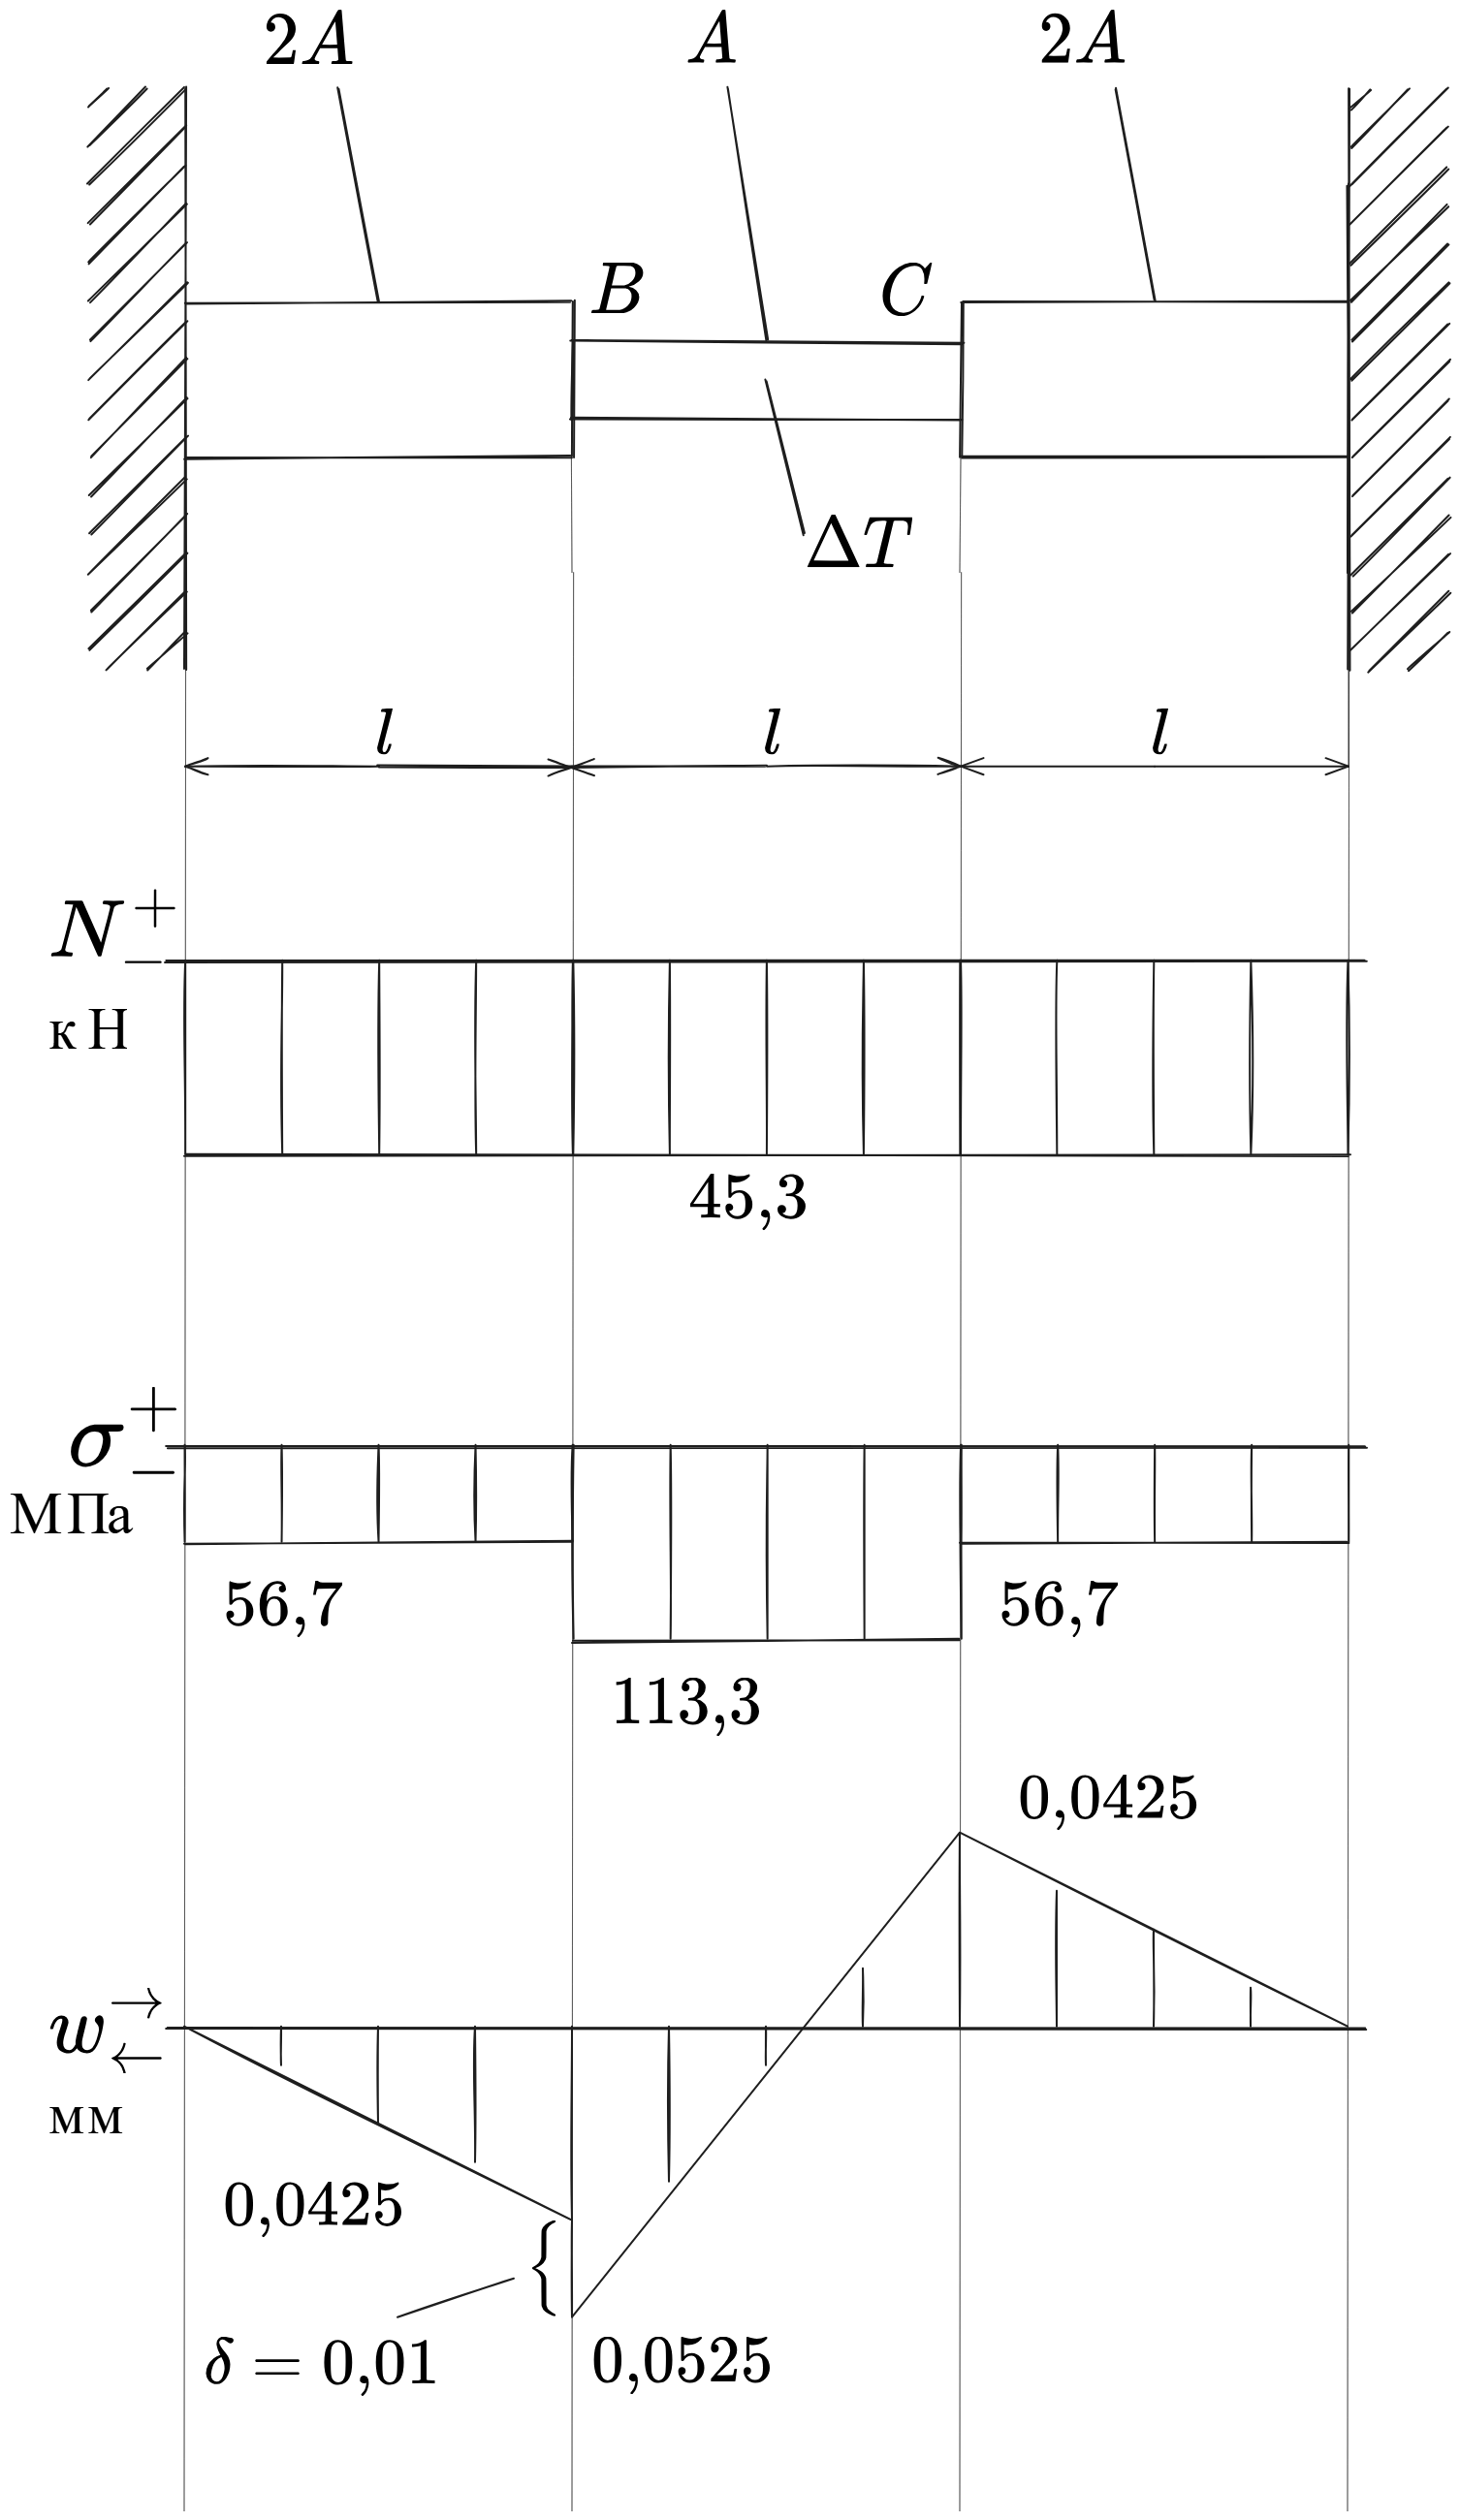
\includegraphics[
    width=0.90\linewidth,
    height=0.8\textheight,
    keepaspectratio
  ]{figures/task2_apure.png}
\end{center}

\heading{ОТВЕТ}

При $\sigma_{\max}=100\,\text{МПа}$:
\(\qquad
{\delta=0{,}03\,\text{мм}}
\)
% ===== ЗАДАЧА 3 =====
\clearpage
\heading{ЗАДАЧА 3}
\heading{УСЛОВИЕ}
Определить нагрузку, при которой в стержневой системе возникают первые пластические деформации.
Найти напряжения, возникающие в стержнях при найденной нагрузке.
\begin{equation*}
  l=200\,\text{мм},\quad
  A=300\,\text{мм}^2,\quad
  E=10^5\,\text{МПа},\quad
  \sigma_{\text{т}}=160\,\text{МПа}.
\end{equation*}
\begin{center}
  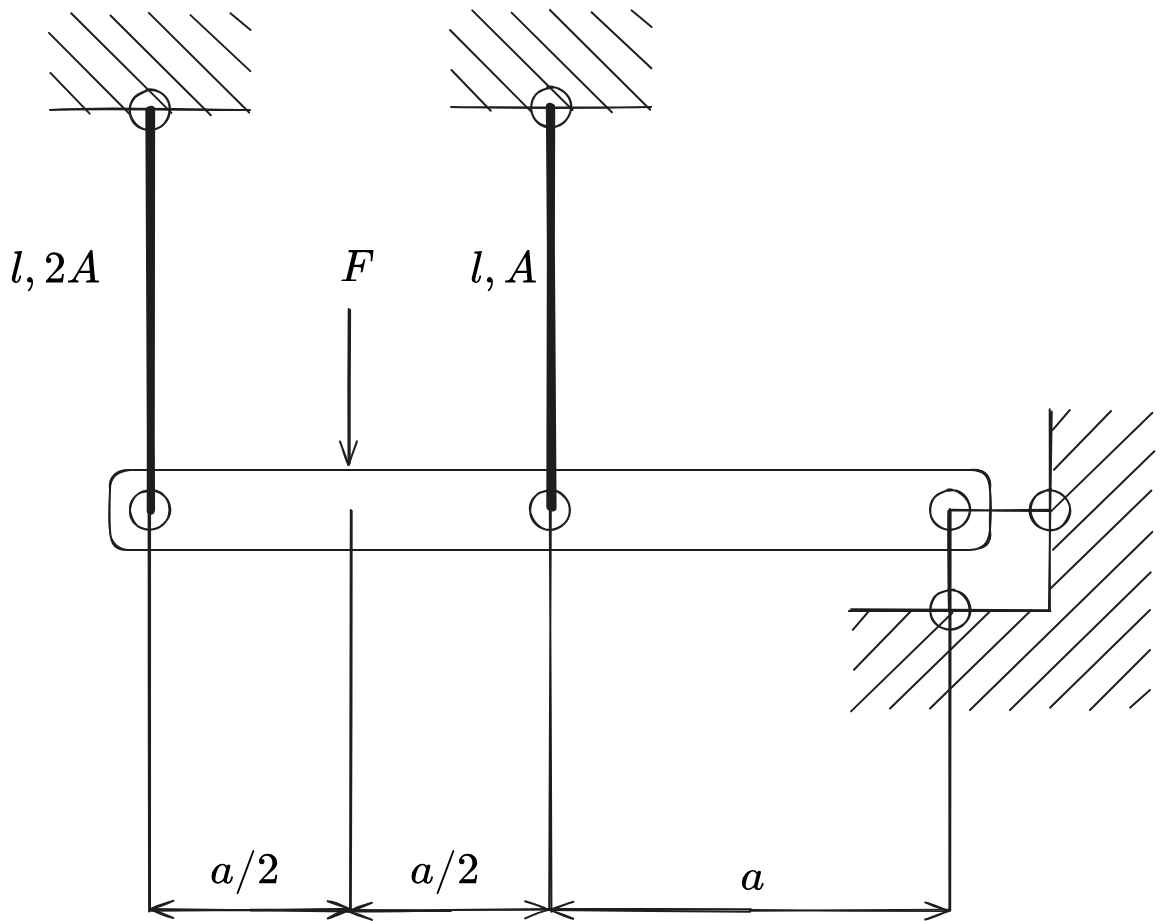
\includegraphics[
    width=0.90\linewidth,
    height=0.50\textheight,
    keepaspectratio
  ]{figures/task3_conditions.png}
\end{center}
\clearpage
\heading{РЕШЕНИЕ}
\setcounter{solutionstep}{0}

\step{Уравнение моментов}
\begin{center}
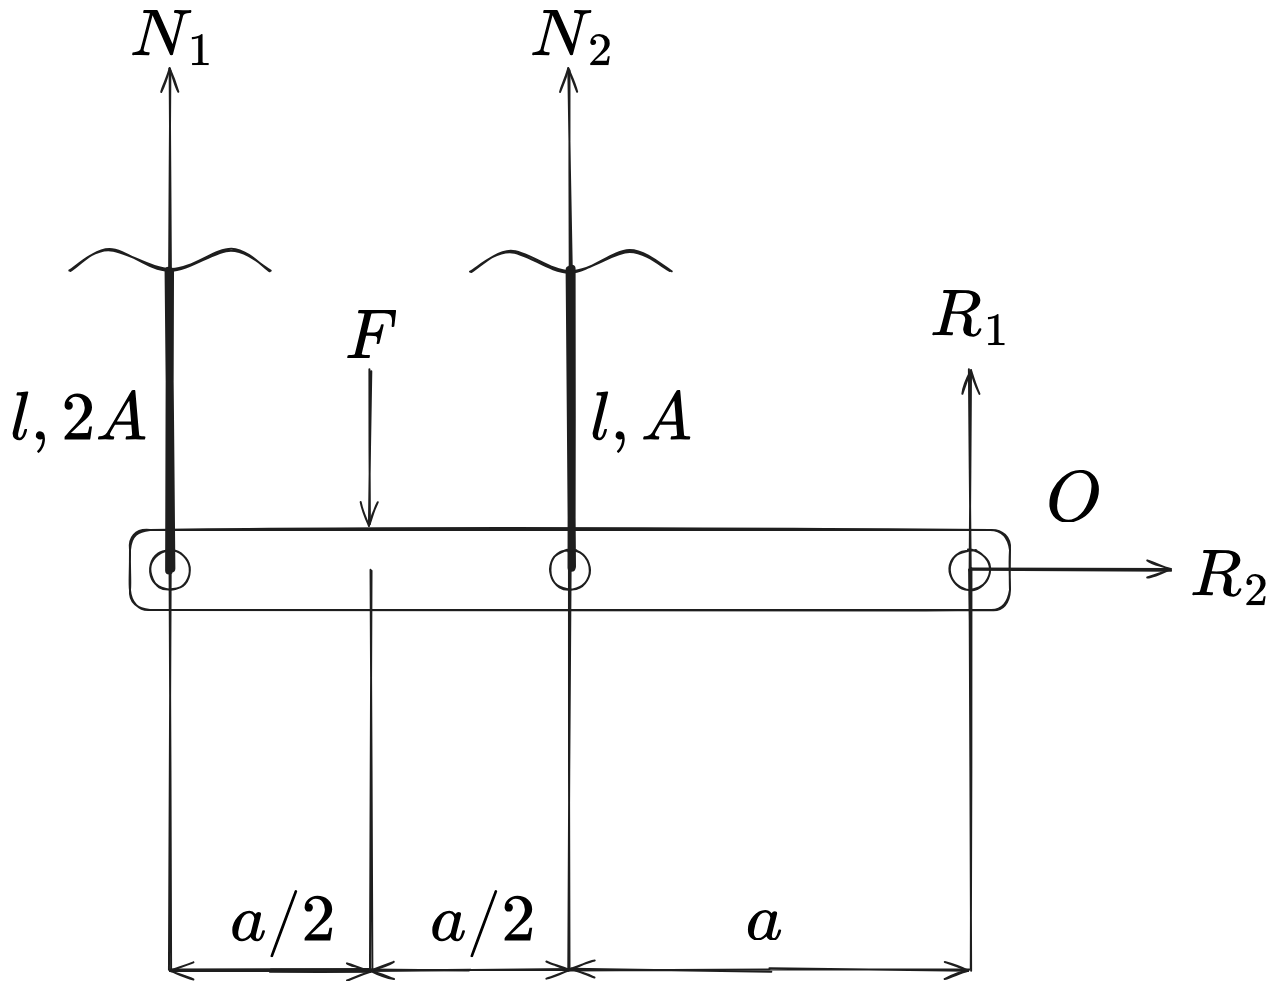
\includegraphics[
width=0.90\linewidth,
height=0.34\textheight,
keepaspectratio
]{figures/task3_ISF.png}
\end{center}
\begin{gather*}
\sum M_O=-N_1\cdot2a+F\cdot\frac{3}{2}a-N_2\cdot a=0\\
\frac{2}{3}N_2+\frac{4}{3}N_1=F
\end{gather*}

\step{Определение сил и изменения длины}
\begin{center}
  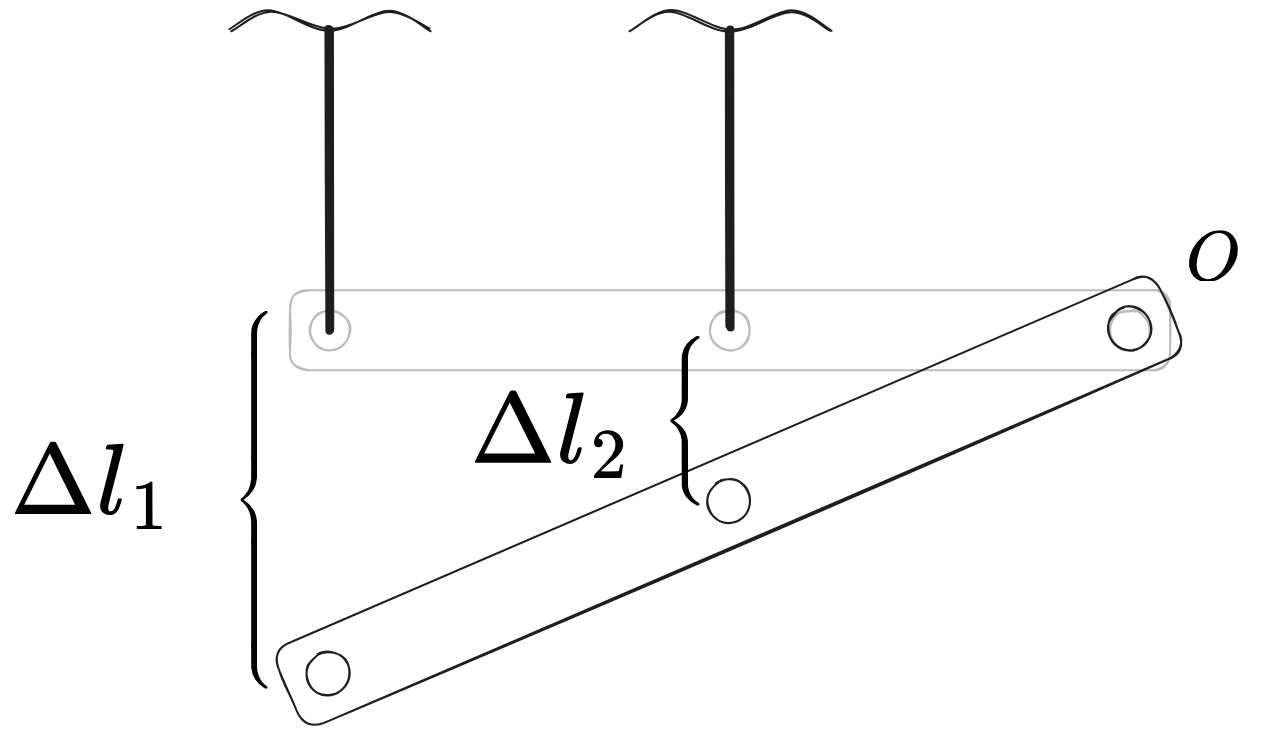
\includegraphics[
    width=0.90\linewidth,
    height=0.15\textheight,
    keepaspectratio
  ]{figures/task3_compatability.png}
\end{center}

\begin{align*}
\Delta l_1&=2\Delta l_2\\
\frac{N_1l}{2EA}&=2\frac{N_2l}{EA}\\
N_1&=4N_2\\
N_1&=\frac{2}{3}F\\
N_2&=\frac{1}{6}F
\end{align*}


\step{Определение напряжений}
\begin{align*}
\sigma_1&=\frac{N_1}{2A}=\frac{F}{3A}\\
\sigma_2&=\frac{N_2}{A}=\frac{F}{6A}
\end{align*}

\step{Определение нагрузки \(F_\text{т}\), при которой начинаются первые пластические деформации}

Пластические деформации возникают, когда напряжение хотя бы в одном из стержней достигает предела текучести материала. Так как \(\sigma_1\geq\sigma_2\) то они возникают в 1 стержне когда:
\begin{align*}
\sigma_1&=\sigma_\text{т}\\
\frac{1}{3}\frac{F}{A}&=\sigma_\text{т}\\
F_{\text{т}}&=3\sigma_\text{т} 
\end{align*}

\step{Определение величины нагрузки и напряжений при найденной нагрузке}


\begin{equation*}
  F_{\text{т}}=3A\sigma_{\text{т}}
  =3\cdot300\,\text{мм}^2\cdot160\,\text{МПа}=144000\,\text{Н}.
\end{equation*}


\begin{equation*}
  \sigma_1=\frac{F_{\text{т}}}{3A}
  =\frac{144000\,\text{Н}}{3\cdot300\,\text{мм}^2}
  =160\,\text{МПа}.
\end{equation*}

\begin{equation*}
  \sigma_2=\frac{F_{\text{т}}}{6A}
  =\frac{144000\,\text{Н}}{6\cdot300\,\text{мм}^2}
  =80\,\text{МПа}.
\end{equation*}

\heading{ОТВЕТ}

\begin{equation*}
  F_{\text{т}}=144000\,\text{Н},\qquad
  \sigma_1=160\,\text{МПа},\qquad
  \sigma_2=80\,\text{МПа}.
\end{equation*}

Первые пластические деформации возникают в левом стержне.

\end{document}